\begin{frame}{Double objectif}
	%	\begin{figure}
		%		\centering
		%		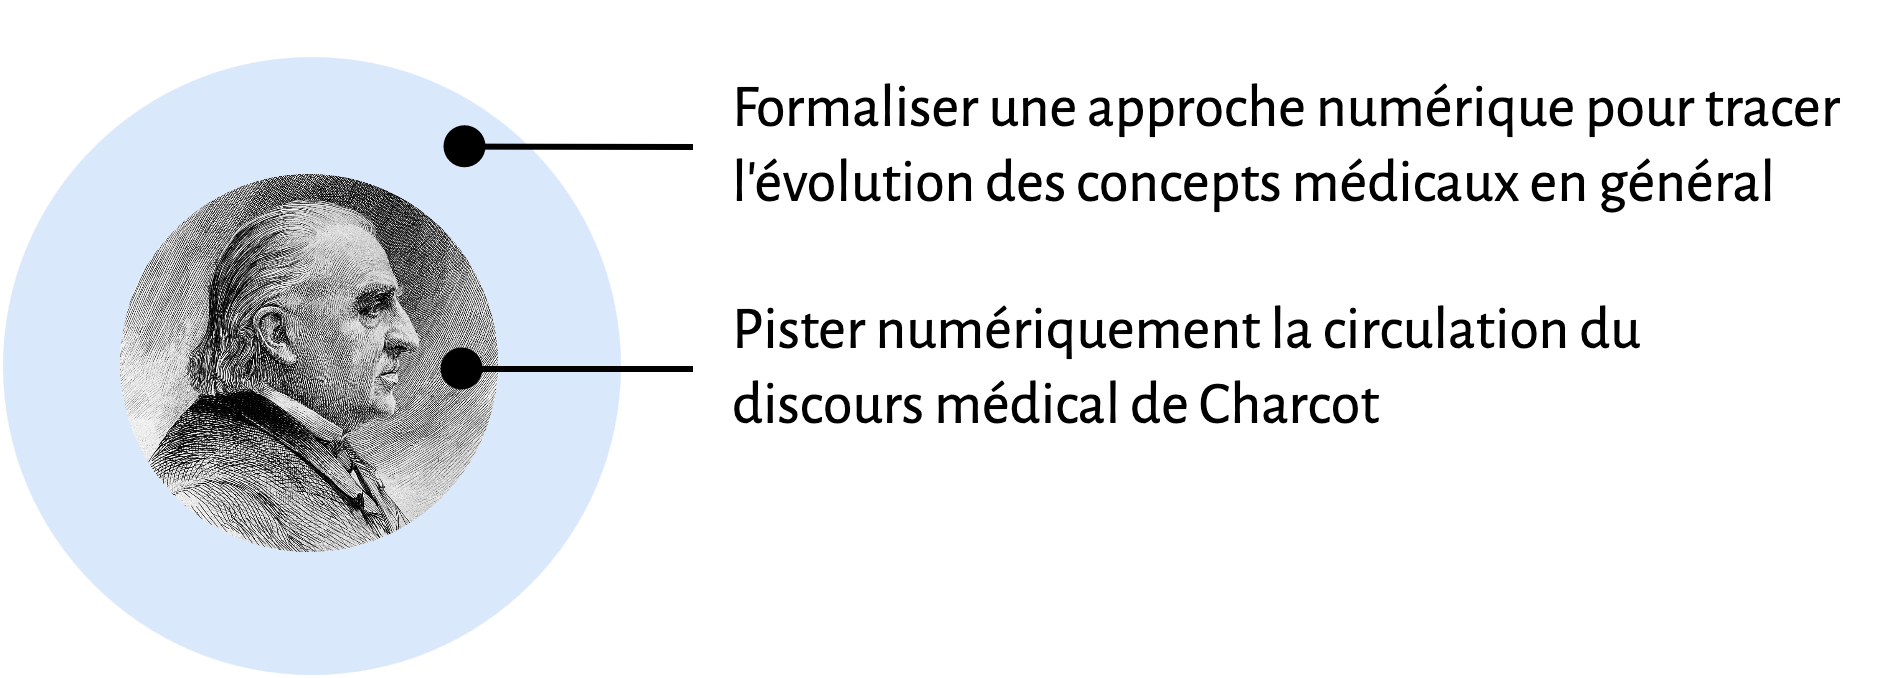
\includegraphics[width=1\textwidth]{pic/objectif_double.png}
		%		%\caption{}
		%	\end{figure}
	%	
	%	\begin{variableblock}{}{bg=white,fg=RubineRed}{bg=green,fg=red}
		%		\centering
		%		%Comment mesurer l'impact de Charcot sur son réseau scientifique ?
		%		Quels sont les concepts médicaux introduits ou transmis par Charcot qui ont eu un impact sur son réseau scientifique ?
		%	\end{variableblock}
	%	
	%	%{\footnotesize ensembles de mots liés par leur sémantique, traitant d'un domaine commun, p. ex. neurologie.}
%	Enjeu de recherche : comment les savoirs scientifiques ont été transmis la littérature médicale du \textsc{XIX}\ieme{} et \textsc{XX}\ieme{} siècle.
	\begin{tikzpicture}
		% Cercle bleu de fond
		\fill[orange!20] (0,0) circle (2.0);
		
		% Image de Charcot dans un cercle
		\node[anchor=center, circle, inner sep=0pt, minimum size=5cm, path picture={
			\node at (path picture bounding box.center){
				\includegraphics[width=2.5cm]{pic/charcot\_profil-modified.png}
			};
		}] at (0,0) {};
		
		% Points noirs
		\fill (1.1,1.1) circle (3pt);
		\fill (1.0,-0.5) circle (3pt);
		
		% Lignes
		\draw[thick] (1.1,1.1) -- (2.2,1.1);
		\draw[thick] (1.0,-0.5) -- (2.2,-0.5);
		
		% Textes (avec taille réduite et text width pour retour à la ligne)
		\node[anchor=west, align=left, text width=6cm, font=\small] at (2.3,1.1) {
			Formaliser une approche numérique pour tracer l'évolution des concepts en général
		};
		
		\node[anchor=west, align=left, text width=6cm, font=\small] at (2.3,-0.5) {
			Pister numériquement la circulation des concepts médicaux associés à Charcot
		};
		
	\end{tikzpicture}
	
%\textcolor{blue}{*} : 
%	\begin{block}{}
%				\centering
%				%Comment mesurer l'impact de Charcot sur son réseau scientifique ?
%				\textcolor{red}{Quels concepts médicaux associés à Charcot ont-ils eu un impact significatif sur son réseau\textcolor{blue}{*} scientifique du point de vue computationnel ?}
%
%			\end{block}
%			\begin{flushright}
%				\footnotesize
%				\textcolor{blue}{*} élèves, collègues et successeurs $\rightarrow$ collaborateurs
%			\end{flushright}
			
%	\begin{block}{}
%		Est-il possible de mesurer l'impact de Charcot sur son réseau* scientifique en s’appuyant sur les termes scientifiques qu'il a employés ?
%	\end{block}
\begin{enumerate}
	\item définir le terme \textit{concept scientifique} du point de vue de \textsc{TAL}
	\begin{itemize}
		\item concept ? idée ? terme ? mot ? mot-clé ? entité nommée ?
	\end{itemize}
	\item comment des concepts circulent d’une discipline à une autre
%	\begin{flushright}
%		\small
%		\citep[p.~331]{landais2014frederic}
%	\end{flushright} 
%	\item mesurer l'impact de Charcot sur l'histoire des neurosciences à travers les termes scientifiques qu'il a employés et qui ont été repris par son réseau scientifique.
\end{enumerate}


\end{frame}